\documentclass[tikz,border=10pt]{standalone}
\begin{document}
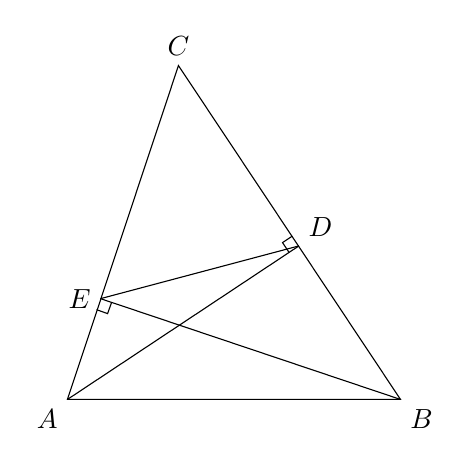
\begin{tikzpicture}
\coordinate (A) at (0,0);
\coordinate (B) at (4.23,0);
\coordinate (C) at (1.41,4.24);
\coordinate (E) at (0.42,1.28);
\coordinate (D) at (2.94,1.95);

\draw (A) -- (B) -- (C) -- cycle;
\draw (A) -- (D);
\draw (E) -- (D);
\draw (E) -- (B);

\draw (0.37,1.14) -- (0.51,1.09) -- (0.56,1.23);
\draw (2.857,2.075) -- (2.732,1.992) -- (2.815,1.867);

\node[below left] at (A) {$A$};
\node[below right] at (B) {$B$};
\node[above] at (C) {$C$};
\node[left] at (E) {$E$};
\node[above right] at (D) {$D$};
\end{tikzpicture}
\end{document}
